\documentclass[12pt]{article}
\usepackage[T2A]{fontenc}
\usepackage[utf8]{inputenc}
\usepackage{multirow}
\usepackage{caption}
\usepackage{subcaption}
\usepackage{amsmath}
\usepackage{amssymb}
\usepackage{changepage}
\usepackage{graphicx}
\usepackage{float}
\usepackage[english,russian]{babel}
\usepackage{amsmath, amsfonts, amssymb, amsthm, mathtools}
\usepackage{xcolor}
\usepackage{array}
\usepackage{hyperref}
\usepackage{physics}
\usepackage[top = 1.5cm, left = 1.5 cm, right = 1.5 cm, bottom = 3 cm]{geometry}
\usepackage{import}
\usepackage{xifthen}
\usepackage{pdfpages}
\usepackage{transparent}

\newcommand{\incfig}[1]{
    \import{./figures/}{#1.pdf_tex}
}

\title{Матан первая домашка.}
\author{Шахматов Андрей, Б02-304}
\date{\today}

\begin{document}
\maketitle
\tableofcontents

\section{T1}
$$f(x, y) = \sqrt{xy}$$
Тогда область определения $D_f = \{(x, y) \mid (x, y) \in \mathbb{R}^2 \, (x \leq 0 \, \land y \leq 0) \lor (x \geq 0 \, \land y \geq 0)\}$
\begin{figure}[H]
    \centering
    \def\svgwidth{0.7\columnwidth}
    \incfig{T1_1}
    \caption{Область определения функции}
    \label{fig:T1_1}
\end{figure}
Область опредлеения будет замкнутым множеством, так как совпадает со своим замыканием. 
Из рисунка \ref{fig:T1_1} видно, что множество не является выпуклым, однако является линейно свзяным, ведь любые 2 точки можно соединить кривой проходящей через точку (0, 0).
$$f(x, y) = \frac{1}{x^4 + y^4 - 1}$$
Область определения данной функции $D_f = \{(x, y) \mid (x, y) \in \mathbb{R}^2 \, x^4 + y^4 \ne 1 \}$
\begin{figure}[H]
    \centering
    \def\svgwidth{0.7\columnwidth}
    \incfig{T1_2}
    \caption{Область определения функции}
    \label{fig:T1_2}
\end{figure}
Областью определения является всё пространство кроме кривой $x^4 + y^4 = 1$. Так как такая кривая является замкнутой, то её дополнение открыто,
а значит область определения открыта. Также область определения не является выпуклой, связной или линейно связной, так как разбивается кривой на два открытых непересекающихся
множества.
$$f(x, y) = \ln(1 - 2x - x^2 - y^2)$$
Тогда область определения $D_f = \{(x, y) \mid (x, y) \in \mathbb{R}^2 \, x^2 + y^2 < 1 - 2x\}$.
Решим полученное неравенство $x^2 + 2x + 1 + y^2 < 2$, что эквивалентво $(x + 1)^2 + y^2 < \sqrt{2}^2$, 
что соответствует открытому шару радиуса $\sqrt{2}$ с центром в точке $(-1, 0)$.
\begin{figure}[H]
    \centering
    \def\svgwidth{0.7\columnwidth}
    \incfig{T1_3}
    \caption{Область определения функции}
    \label{fig:T1_3}
\end{figure}

Так как область определения - открытый шар, то она открыта. Также область определения связна, линейно связна и выпукла.
\section{T2}
$$M = \{(e^t \cos{t}, e^t \sin{t}) \mid t \in \mathbb{R}\}$$
Данное множество является образом непрерывной кривой, потому оно линейно свзяно (любые две точки можно соединить данной кривой), потому $M$ - связно.
Данное множество не является открытым, поскольку содержит некоторые свои граничные точки. 
При этом замыкание множества содержит точку $(0, 0)$, однако сама кривая её не содержит, так как $R = \sqrt{x^2 + y^2} = e^t > 0$, что 
означает незамкнутость $M$.
\begin{figure}[H]
    \centering
    \def\svgwidth{0.4\columnwidth}
    \incfig{T2_graph}
    \caption{График кривой}
    \label{fig:T2}
\end{figure}
\section{T3}
$$M = {(x_1, x_2, x_3, x_4) \in \mathbb{R}^4 \mid x_1^2 + x_2^2 + x_3^2 < x_4^2}$$
Рассмотрим функцию $g:\mathbb{R}^4 \to \mathbb{R},\, g(x_1, x_2, x_3, x_4) = x_4^2 - x_1^2 + x_2^2 + x_3^2$, такая функция является непрерывной. Рассмотрим прообраз множества
$g^{-1}(Q), \, Q = (0, +\infty)$, при этом прообраз равен исследуемому множеству $M$. По топологическому
определению непрерывности прообраз открытого $Q$ открыт, а значит $M$ - открыто. Также множество $M$ не является линейно свзяным, так как
все кривые, соединяющие точки с координатами $x_4$ разных знаков должны проходить через точку с координатой $x_4 = 0$, которая не содержится в множестве $M$.
Тогда так как $M$ - открыто и не линейно связно, то оно не связно.
\section{T5}
Нужно доказать, что $\bigcap_{n \in \mathbb{N}}^{\infty}B_0\left(\frac{1}{n}\right) = \{0\}$.
С одной стороны $\forall k \in \mathbb{N} \, 0 \in B_0\left(\frac{1}{k}\right) \Rightarrow \{0\} \subseteq \bigcap_{n \in \mathbb{N}}^{\infty}B_0\left(\frac{1}{n}\right)$.
С другой стороны рассмотрим множество $A = \mathbb{R} \setminus \{0\}$, для любого $a \in A$
существует $k$ такое что $\frac{1}{k} < |a|$, а значит $a \not \in B_0\left(\frac{1}{k}\right) \Rightarrow \bigcap_{n \in \mathbb{N}}^{\infty}B_0\left(\frac{1}{n}\right) \not \in A \Rightarrow B_0\left(\frac{1}{k}\right) \Rightarrow \bigcap_{n \in \mathbb{N}}^{\infty}B_0\left(\frac{1}{n}\right) \in \{0\}$. Тогда через двойное включение получаем требуемый факт.
\section{T6}
Рассмотрим множество значений последовательности Гейне $a_n \rightarrow 0$. Данное множество не будет замкнутым, так как
его замыкае будет содержать $0$, но ни один из членов последовательности не равен $0$. А также каждая точка данного множества является членом последовательности $a_n$ и потому изолирована.
\section{2.39}
Рассмотрим две последовательности Гейне $x_n \to x_0$ и $y_k \to y_0$. Требуется доказать, что при условии
$$\lim_{n \to \infty} f(x_n, y_k) = B(y_k)$$ и $$\lim_{n \to \infty} f(x_n, y_n) = A$$ следует, что $$\lim_{k \to \infty} B(y_k) = A$$.
В силу существования первых двух пределов для достаточно больших $n, k$ выполняется:
$$|f(x_n, y_n) - A| < \epsilon$$
$$|f(x_n, y_k) - B(y_k)| < \epsilon$$
$$|f(x_n, y_k) - f(x_k, y_k)| < \epsilon$$
Последнее неравенство выполняется в силу фундаментальности последовательности $f(x_n, y_k)_n$.
Рассмотрим $|B(y_k) - A| < |B(y_k) - f(x_n, y_k)| + |f(x_n, y_k) - f(x_k, y_k)| + |f(x_k, y_k) - A| < 3\epsilon$. Что означает
$$\lim_{k \to \infty} B(y_k) = A$$
\section{Т10}
Пусть существует $g:\mathbb{R}^2 \to \mathbb{R}$ и $g$ - непрерывна и инъективна. Рассмотрим сужение $g_y: \mathbb{R} \to \mathbb{R}$, $g_y(x) = g(x, y)$.
Тогда $g_y$ также непрерывна, а значит он переводит связные множества в связные, из чего следует $g_y(\mathbb{R}) = Q(y)$, где $Q(y)$ - отрезок, интервал или полуинтервал.
Тогда так как $g$ - инъективна выполняется: $\mathbb{R} = \bigsqcup_{y \in \mathbb{R}} Q(y)$.
Докажем промежуточную лемму: инъёктивная и непрерывная функция монотонна. Предположим противное:
$\exists x_1 < x_2 < x_3 \mid f(x_1) < f(x_2) > f(x_3) \lor f(x_1) > f(x_2) < f(x_3)$, строгие знаки 
получены с учётом инъёктивности. Без ограничения общности рассмотрим первый вариант $f(x_1) < f(x_2) > f(x_3)$.
Пусть $f(x_3) > f(x_1)$, тогда по теореме о промежуточных значениях существует $x \in (x_1, x_2) \mid f(x) = f(x_3)$, 
тогда так как $x < x_3 \Rightarrow x \not = x_3$, но $f(x) = f(x_3)$ - противоречие с инъективностью.
Тогда оказывается, что каждая из $g_y$ - монотонна. Так как функция $g_y$ монотонна то по теореме об обратной
функции обратная $f^{-1}$ - непрерывна, а значит $f$ переводит открытые в открытые. А значит все множества
$Q(y)$ - интервалы. Тогда так как из покрытия открытого множества интервалами можно выбрать счётное подпокрытие $\mathbb{R} = \bigsqcup_{n \in \mathbb{N}} Q(y_n)$.
Но тогда мы получили дизъюнктное разбиение действительной прямой непустыми интервалами - противоречие со связностью.
\section{T11}
Построим кривую Пеано. Рассмотрим отрезок \([0, 1]\) и квадрат \([0, 1]^{2} \). 
Будем итеративно строить разбиения: на первом шаге разобьём отрезок на 4 равных отрезка, а квадрат
на 4 равных квадрата, на втором разобьём квадрат на 16 квадратов и отрезок на 16 отрезков. Согласно
Рис. \ref{fig:T11} сопоставим отрезкам соответствующие квадраты. 
\begin{figure}[H]
    \centering
    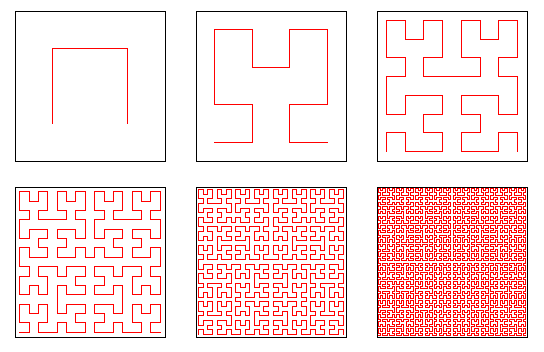
\includegraphics[width=0.8\textwidth]{figures/Hilbert_curve.png}
    \caption{Обходы для квадратов 1 - 6 уровня.}
    \label{fig:T11}
\end{figure}
Выберем точку из отрезка. Если точка не принадлежит 2 отрезкам никакого уровня, для каждого 
уровня разбиения отрезка получим соответствие отрезка, к которому принадлежит точка и квадрата. 
Тогда получаем что каждой точке соответствует последовательность вложенных стягивающихся квадратов. 
Их общая точка и будет образом точки отрезка. 
В случае если на каком-то шаге точка из отрезка принадлежит 2 подотрезкам, они обязательно будут 
связаны к квадратами с общей стороной (из построения обхода), тогда будем рассматривать прямоугольники,
образованные данными квадратами, они также стягиваются и точка их пересечения - образ точки отрезка.
Повторяя аналогичные рассуждения в обратном порядке получим, что исследуемое отображение сюрьективно.
Докажем непрерывность отображения. Для точки выберем квадрат, полностью лежащий в заданной эпсилон окрестности. 
рассмотрим отрезок, соответствующий данному квадрату. Все точки из этого отрезка будут лежать в этом квадрате, так как 
близким отрезкам соответствуют близкие квадраты (обход такой).

Теперь пусть такое отображение называется $g: [-\frac{\pi}{2}, \frac{\pi}{2}] \to [-\frac{\pi}{2}, \frac{\pi}{2}]^2$, тогда 
применяя к функции гомеоморфизм арктангенса слева и покоординатный тангенс слева получим непрерывное отображение 
из $\mathbb{R} \to \mathbb{R}^2$.

\section{T12}
(б)
\[
    \begin{dcases}
        \exp{-\frac{1}{x^{2} + y^{2}}}, (x, y) \not = (0, 0)\\
        0, (x, y) = (0, 0)\\
    \end{dcases}
\]
Найдём частные производные:
\[
    \partial_x f(0, 0) = \lim_{x \to 0}{\frac{\exp{-\frac{1}{x^2}}}{x}} = 0 
\]
\[
    \partial_y f(0, 0) = \lim_{y \to 0}{\frac{\exp{-\frac{1}{x^2}}}{y}}{y} = 0
\]
Проверим дифференцируемость функции:
\[
    \frac{1}{\rho }\vert \exp{-\frac{1}{{h^1}^{2} + {h^2}^{2}  }} \vert = \frac{1}{\rho }\vert \exp{-\frac{1}{\rho^{2} }} \vert \to 0, \rho \to 0
\]
(в)
\[
    f(x, y) = \ln(1 + \sqrt[3]{x^{2} y})
\]
Частные производные равны нулю: 
\[
    \vert \frac{1}{\rho }\ln(1 + \sqrt[3]{x^{2} y}) \vert = \vert \frac{1}{\rho }\ln(1 + \rho \sqrt[3]{\cos^{2}{\phi} \sin \phi}) \vert
\]
Предел такого выражения зависит от напрвдения, например при \(\phi = 0\) предел равен 0, а при других углах \(1\). Тогад разность приращения и дифференциала
не равна \(o(\rho )\), что недифференцируемость функции.   

\section{T14}
\[
    f(x, y, z) = (1 + x)^\alpha(1 + y)^\beta(1 + z^\gamma)
\]
\[
    \ln{f(x, y, z)} = \alpha\ln(1 + x) + \beta\ln(1 + y) + \ln(1 + z^\gamma)
\]
\[
    d \ln{f(x, y, z)} = \frac{d f(x, y, z)}{f(x, y, z)} = \frac{\alpha dx}{1 + x} + \frac{\beta dy}{1 + y} + \frac{\gamma z^{\gamma - 1}dz}{1 + z^{\gamma} }
\]
\[
    d f(0, 0, 0) = \alpha dx + \beta dy
\]
\[
    d^2 f(x, y, z) = d \left( f(x, y, z) \cdot d \ln{f(x, y, z)} \right) = d f(x, y, z) \otimes d \ln{f(x, y, z)} + f(x, y, z) \cdot d^2 \ln{f(x, y, z)} 
\]
Первое слагаеемое:
\[
    d f(0, 0, 0) \otimes d \ln{f(0, 0, 0)} = (\alpha dx + \beta dy)^{2}
\]
Второе слагаемое:
\[
    d^2 \ln{f(x, y, z)} = -\frac{\alpha dx^{2}}{(1 + x)^{2}} - \frac{\beta dy^{2}}{(1 + y)^{2}} + \frac{\gamma (\gamma - 1) z^{\gamma -2} - \gamma z^{2\gamma -2}}{(1 + z^{\gamma})^{2} }
\]
Тогда второй дифференциал в нуле равен:
\[
    d^2 f(0, 0, 0) = (\alpha dx + \beta dy)^{2} - \alpha dx^{2} - \beta dy^{2} = (\alpha^{2} - \alpha)dx^{2}  + (\alpha ^{2} -\alpha ^{2} )dy^{2} + 2\alpha \beta dx \otimes dy
\]
\section{T15}
(а)
\[
    ef = e^{x - y + f}
\]
\[
    e df = (dx - dy + df) ef \implies df = \frac{f}{1 - f}(dx - dy) 
\]
\[
    d^2f = df \otimes (dx - dy + df) + f d^2 f + df^2
\]
\[
    d^2 f = \frac{1}{1 - f}(2df^2 + df \otimes dx - df \otimes dy)
\]
\\
б)
\[
    f^3 - 3xyf - 2 = 0, f(1, 1) = 2
\]
\[
    3f^2 df - 3yf dx - 3xf dy - 3xy df = 0 \implies df = \frac{dx + dy}{f^2 - xy}
\]
Значение \(df(1, 1) = \frac{dx + dy}{3}\) 
\[
    d^2 f = d \left( \frac{1}{f^2 - xy} \right) \otimes (dx + dy) 
\]
\[
    d \left( \frac{1}{f^2 - xy} \right) = -\frac{2f df - ydx - x dy}{(f^2 - xy)^2} = -\frac{4df - dx - dy}{9}
\]
\[
    d^2 f(1, 1) = (dx + dy) \otimes -\frac{\frac{4}{3}dx + \frac{4}{3}dy - dx - dy}{9} = \frac{1}{27}(dx + dy)^2 
\]
Тогда частные производные одинаковы и равны: \(\frac{1}{27}\). 
\section{T16}
\[
    f(x, y, z) = \ln{x + y + z} = \ln g
\]
\[
    d^n f(x, y, z) = \partial_{g^n} f \cdot dg^n = \frac{(-1)^{n - 1} (n - 1)!}{(x + y + z)^n} \cdot (dx + dy + dz)^n
\]
То есть все частные производные равны между собой и равны: \(\frac{(-1)^{n - 1} (n - 1)!}{(x + y + z)^n}\). 
\section{T17}
a) 
Нужно доделать))).
\[
    f(x, y) = (1 + x)^y = e^{y\ln (1 + x)} 
\]
\[
    df = (1 + x)^y (dy\ln(1 + x) + \frac{ydx}{1 + x})
\]
Тогда $df(0, 0) = 0$.
\[
    d^2 f = df \otimes (dy\ln(1 + x) + \frac{ydx}{1 + x}) + f(x, y) (dy \otimes \frac{dx}{1 + x} + dx \otimes \frac{dy(1 + x) - ydx}{(1 + x)^2})
\]
Тогда $d^2 f(0, 0) = 2 dy \otimes dx$ 
\[
    f(h) = 1 + h^1 h^2 + o(||h||^2)
\]
\section{T18}
\[
    \sum_{n=1}^{N} \frac{2n + 1}{n^2(n+1)^2} = \sum_{n=1}^{N} \frac{1}{n^2} - \frac{1}{(n+1)^2} = 
    1 - \frac{1}{(N+1)^2} \to 1, N \to 0 
\]
\section{T19}
\[
    \sum_{n=1}^{\infty} e^{\alpha n}n^\beta 
\]
Воспользуемся критерием Коши:
\[
    \lim_{n \to \infty} \sqrt[n]{e^{\alpha n}n^\beta} = 
    \lim_{n \to \infty} e^\alpha (n^{\frac{1}{n}})^\beta = 
    e^\alpha 
\]
При $\alpha > 0$ ряд расходится, при $\alpha < 0$ ряд сходится. Рассмотрим случай $\alpha = 0$:
\[
    \sum_{n=1}^{\infty} e^n n^\beta 
\]
Но так как экспонента растёт быстрее степени, то не выполняется необходимое условие сходимости, а занчит ряд расходится. 
\section{T20}
а)
\[
    \sum_{n=1}^{\infty} \ln (1 + \frac{1}{n^{\frac{3}{2}}}) < \sum_{n=1}^{\infty} \frac{1}{n^{\frac{3}{2}}}
\]
Так как ряд $\sum_{n=1}^{\infty} \frac{1}{n^{\frac{3}{2}}}$ - сходится абсолютно, то и исходный ряд сходится абсолютно.\\
в)
\[
    \sum_{n=1}^{\infty} \frac{(2n)!!}{n!} \arctg \frac{1}{3^n} < \sum_{n=1}^{\infty} \frac{(2n)!!}{n! 3^n}
\]
Воспользуемся признаком Даламбера:
\[
    q = \lim_{n \to \infty} \frac{2n + 2}{n + 1} \frac{1}{3} = \frac{2}{3}
\]
Так как $q < 1$ то исходный ряд сходится абсолютно. \\
г) 
\[
    \sum_{n=1}^{\infty} \left( \frac{n^2 + 5}{n^2 + 6} \right)^{n^3}
\]
Воспользуемся критерием Коши:
\[
    q = \lim_{n \to \infty} \left( \frac{n^2 + 5}{n^2 + 6} \right)^{n^2} = \lim_{n \to \infty} \left( 1 - \frac{1}{n^2 + 6} \right)^{n^{2}} = \frac{1}{e} < 1
\]
Ряд сходится. \\
е)
\[
    \sum_{n=1}^{\infty} \frac{n^n}{(n!)^2}
\]
По признаку Даламбера: 
\[
    q = \lim_{n \to \infty} \frac{(n + 1)^{n+1}}{n^n} \frac{(n!)^2}{(n+1)!^2} = 
    \lim_{n \to \infty} \frac{1}{n+1} (1 + \frac{1}{n})^n = 0
\]
Ряд сходится.
\\
ж)
\[
    \sum_{n=1}^{\infty} (-1)^n \frac{\cos^2 2n}{\sqrt{n}}
\]
По признаку Дирихле: $(-1)^n $ - ограничена. А для достаточно больших $n$ последовательность 
$\frac{\cos ^2 2n}{\sqrt{n} }$ монотонна и стремится к 0. Что означает, что ряд сходится.  
Теперь рассмотрим модуль последовательности:
\[
    \sum_{n=1}^{\infty} \frac{\cos ^2 2n}{\sqrt{n} } = 
    \frac{1}{2}\sum_{n=1}^{\infty} \frac{1}{\sqrt{n}} + \frac{\cos 4x}{\sqrt{n} }
\]
Один из подрядов расходится а второй сходится по тригонометрическому признаку, потому общий ряд тоже расходится.
\\
з) 
\[
    \sum_{n=1}^{\infty} \sin \frac{\sin n}{\sqrt[3]{n}} = \sum_{n=1}^{\infty} \frac{\sin n}{\sqrt[3]{n}} + \frac{\sin^3 n}{6n} + O(\frac{1}{n^{\frac{5}{3}}})
\]
Подсумма с $O(\frac{1}{n^{\frac{5}{3}}})$ сходится абсолютно, подсумма $\frac{\sin n}{\sqrt[3]{n}}$ сходится по тригонометрическому признаку.
\[
    \frac{\sin^3 n}{6n} = \frac{1}{24n} \left( 3\sin x - \sin 3x \right) 
\]
Оба ряда сходятся по тригонометрическому признаку. А значит исходный ряд сходится.
\section{T21}
а)
\[
    \sum_{n=1}^{\infty} \left( \frac{1}{n^\alpha } - \ln (1 + \sin \frac{1}{n}) \right) = \sum_{n=1}^{\infty} \left( \frac{1}{n^\alpha} - \frac{1}{n} + O(\frac{1}{n^{2}}) \right) 
\]
Последовательность из $O(\frac{1}{n^2})$ сходится абсолютно. Тогда рассмотрим первые 2 члена суммы:
\[
    \sum_{n=1}^{\infty} \left( \frac{1}{n^\alpha } - \frac{1}{n} \right) = 
    \sum_{n=1}^{\infty} \left( \frac{1}{n} \left[\frac{1}{n^{\alpha-1} - 1}\right] \right) 
\] 
При $\alpha = 1$ сумма равна $0$ и ряд сходится.
при остальных $\alpha $ сумма расходится.
\\
б)
\[
    \sum_{n=1}^{\infty} \frac{\sin n}{n \ln^\alpha n}
\]
По тригонометрическому признаку ряд сходится при любом $\alpha$, так как $\frac{1}{n \ln ^\alpha n} \to 0, n \to \infty $. 
Доделать)))
\section{T21 доп}
Проверить, что $\sum_{n=1}^{\infty} \sin n\phi$ расходится.
Обозначим частичные суммы $S_n$, тогда: 
\[
    S_n \cdot 2\sin \frac{\phi}{2} = \cos \left( \phi - \frac{\phi}{2} \right)  
    - \cos \left( \phi + \frac{\phi}{2} \right) + \dots = \cos \frac{\phi}{2} - \cos  \phi \left( n + \frac{n}{2} \right) 
\]  
Но тогда сумма расходится, так как предела частичных сумм не существует.
\section{15.33}
По неравенствам Гёльдера и Минковского получим, что последовательность частичных сумм ограничена и возрастает (так как 
последовательности положительные), а значит существует предел частичных сумм - ряд сходится. После перехода к пределу в неравенствах получим неравенство для сумм рядов.
\section{Специальный критерий Коши}

\end{document}